\begin{frame}{%
\begin{minipage}[t]{0.85\textwidth}
Fiskehejre
\end{minipage}%
\hfill
\begin{minipage}[t]{0.1\textwidth}
\raggedleft

\includegraphics[width=0.55cm, height=0.55cm, keepaspectratio]{Billeder/Ikoner/star.png}%
\end{minipage}%
}
\vspace{0.25em}
\begin{columns}[T]
% --- Venstre kolonne: Tekst ---
\column{0.55\textwidth}
\setlength{\parskip}{0.5em}
\small
\RaggedRight\textbf{\textit{Ardea cinerea}} – Særegen storkelignende slank fugl der jager langs kyster, søer, vandløb osv \par

\textbf{Udseende:} \\
\quad – Grå krop med sort nakketop, spidst langt gult næb \par

% --- Højre kolonne: Et billede ---
\column{0.40\textwidth}
\centering
\fbox{%
\begin{minipage}{\linewidth}
\centering
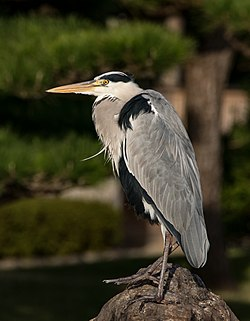
\includegraphics[width=0.8\linewidth, height=10cm, keepaspectratio]{Billeder/Dyr/Fugle/Hejrer/fiskehejre.jpg}
\end{minipage}
}%
\end{columns}
\end{frame}